\section{Aufbau}
\begin{figure}
	\centering
	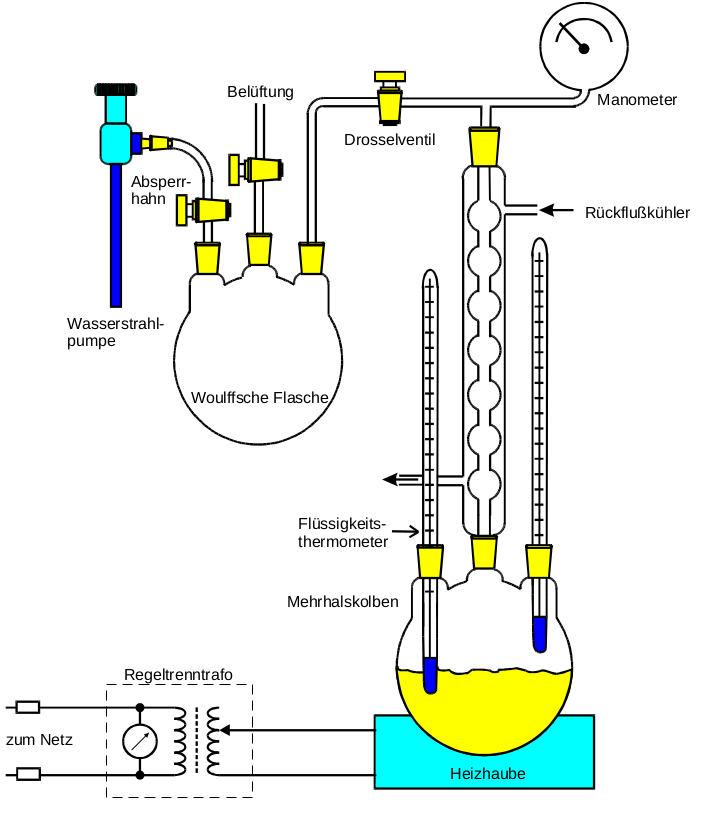
\includegraphics[width=\linewidth-100pt,height=\textheight-100pt,keepaspectratio]{content/Bilder/V203aufbau1.png}
	\caption{Messapparatur zur Aufnahme einer Dampfdruckkurve im Druckbereich von unter $\SI{1}{\bar}$\cite{V203}.}
	\label{fig:Aufbau1}
\end{figure}
\begin{figure}
	\centering
	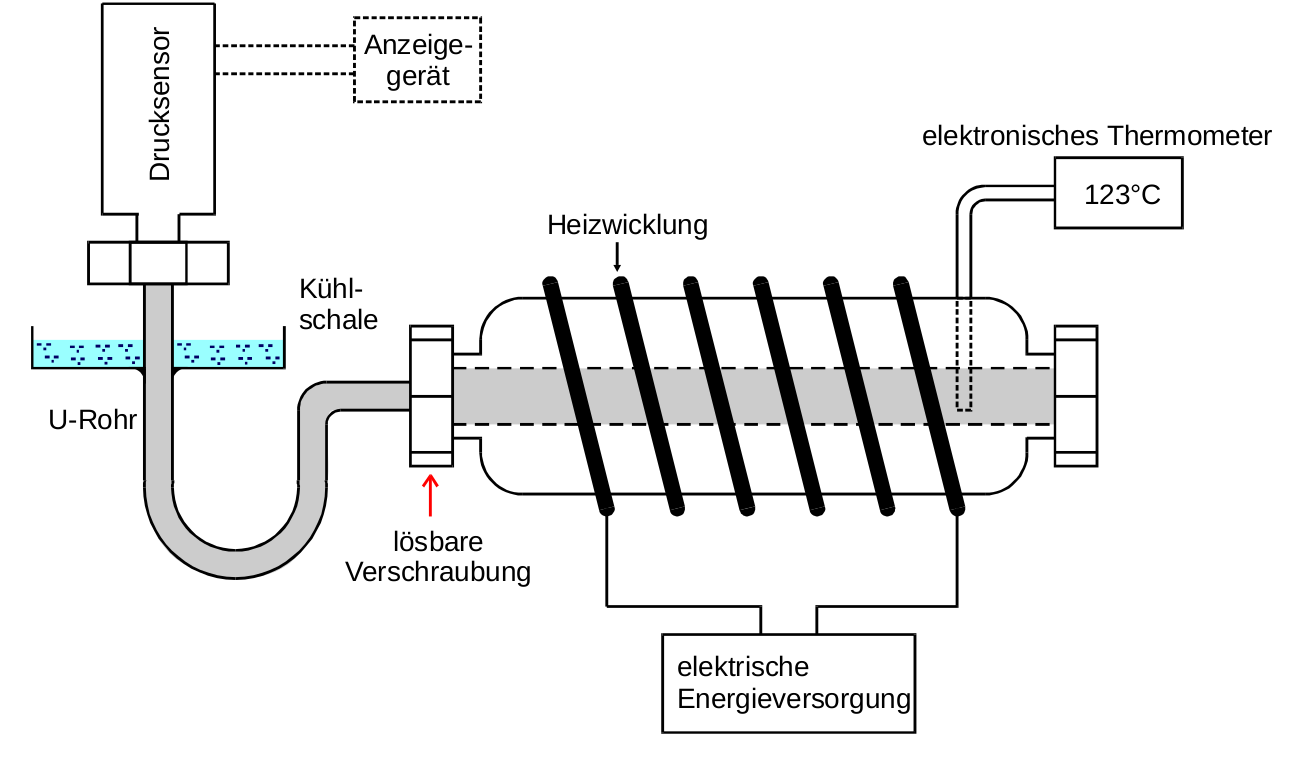
\includegraphics[width=\linewidth-100pt,height=\textheight-100pt,keepaspectratio]{content/Bilder/V203aufbau2.png}
	\caption{Messapparatur zur Aufnahme einer Dampfdruckkurve im Druckbereich von über $\SI{1}{\bar}$\cite{V203}.}
	\label{fig:Aufbau2}
\end{figure}
Zunächst folgt ein Versuchsaufbau zur Aufnahme einer Dampfdruckkurve im Druckbereich
 von unter $\SI{1}{\bar}$. Hierzu wird eine Apperatur der Form aus Abb. \ref{fig:Aufbau1} verwendet.
   Im Zentrum befindet sich ein Mehrhalskolben, welcher mit etwas Wasser gefüllt ist.
    In den äußeren Hälsen befinden sich zwei Flüssigkeitsthermometer, eines um die
     Temperatur des Wassers zu messen und eines für den Raum oberhalb der
      Wasseroberfläche. Der Druck kann über einen elektronischen Druckmesser abgelesen werden.
       Das Wasser kann über eine Heizhaube, welche über einen
       Trenntrafo mit Strom versorgt wird, erhitzt werden. Um ein entweichen
        des auftretenden Wasserdampfes zu verhindern
         wird ein Rückflusskühler oberhalb des Kolbens angebracht, welcher
         ständig von etwas Wasser durchflossen wird, sodass auftretender Dampf
          wieder kondensiert. Der Kolben wird mithilfe einer Wasserstrahlpumpe evakuiert.
           Damit kein Wasser aus dieser in die Apparatur gelangt ist eine
            Woulffsche Flasche zwischengeschaltet. Diese lässt sich über einen
             Absperrhahn in Richtung der Wasserstrahlpumpe und über ein Drosselventil
              in Richtung des Rückflusskühlers verriegeln. Zusätzlich besitzt sie ein Belüftungsventil.

            Um im Anschluss auch eine Dampfdruckkurve im Druckbereich von über
             $\SI{1}{\bar}$ aufzunehmen wird ein Aufbau nach Abb. \ref{fig:Aufbau2} verwendet.
              Dieser besteht aus einem bereits evakuierten und mit etwas Wasser
               gefüllten Gefäß, welches von einer Heizwicklung umschlossen ist.
                Diese wird über eine elektrische Energieversorgung erwärmt. Aus
                 Sicherheitsgründen ist das Gefäß mit einem Metallschutz
                  ummantelt. Die Temperatur im Gefäß wird über ein elektronisches
                   Thermometer abgelesen. Der Druck wird über einen elektronischen
                   Drucksensor bestimmt. Dieser ist über ein U-Rohr mit dem Gefäß
                   verbunden. Er wird über eine Kühlschale gekühlt.
